\section{Durchführung}
\label{sec:Durchführung}

\renewcommand{\labelenumi}{\alph{enumi})}
\begin{enumerate}


\begin{figure}[H]
    \centering
    \begin{subfigure}{0.48\textwidth}
      \centering
      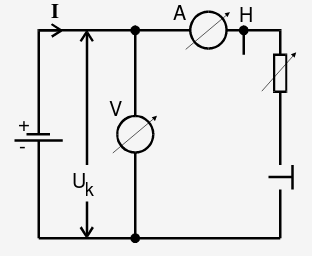
\includegraphics[width=\linewidth-60pt,height=\textheight-60pt,keepaspectratio]{content/Spannungsquelle2.png}
      \caption{{\footnotesize Messungaufbau zur $U_0$ und $R_i$ Bestimmung}}
      \label{fig:Spannung2}
    \end{subfigure}
    \begin{subfigure}{0.48\textwidth}
      \centering
      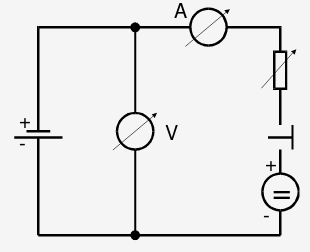
\includegraphics[width=\linewidth-60pt,height=\textheight-60pt,keepaspectratio]{content/Spannungsquelle3.png}
      \caption{{\footnotesize $U_0$ und $R_i $ Bestimmung mit Gegenspannung}}
      \label{fig:Spannung3}
    \end{subfigure}
  \end{figure}


    \item Es wird die Leerlauflaufspannung einer Monozelle mit einem Spannungsmesser ermittelt.
    Es wird der Eingangswiderstand des Voltmeters notiert.

    \item Es wird die Klemmenspannung $U_k$ in Abhängigkeit des Belastungsstroms I mithilfe
    der Schaltung aus Abb. 2 gemessen.
    Hierzu wird der Belastungswiderstand $R_a$ im Bereich von $ 0-50\text{ }\Omega$ variiert.

    \item Es wird eine Gegenspannung wie in Abb. 3 an die Monozelle angelegt, welche ca. $2$ V
    größer als $U_0$ ist. Der Strom fließt nun in umgekehrter Richtung und es gilt:
    \begin{equation}
	    U_k = U_0 + IR_i
    \end{equation}
    Es wird wiederum $U_k$ in Abhängigkeit von $I$ gemessen.

    \item Es soll die Messreihe aus b) nochmals mit dem Sinus bzw. dem
    Rechteckausgang eines RC-Generators durchgeführt werden. Für den Variationsbereich
    von $R_a$ soll gelten:\\
    $1$ V Sinusausgang: $R_a \in [0,1 - 5 $ k$\Omega]$\\
    $1$ V Rechteckausgang: $R_a \in [20 -250\text{ }\Omega]$\\
    Es ist zu beachten das die Messgeräte nur für einen engen Frequenzbereich geeicht sind.
\end{enumerate}
